\section{Unauthenticated user}
\subsection{Sign-up}
A generic user who never logged into the platform can sign up in the platform. To perform this action the user has to click the \textit{sign-in/up} button present in the header\textsubscript{\textbf{G}}.
\begin{figure}[!ht]
    \caption{Sign-in button}
    \vspace{10px}
    
\includegraphics[scale=0.5]{../../../../Images/userManual/signInButton.png}
    \centering
\end{figure}
When the button is pressed the user arrives in the sign-in page here he has to click the \textit{sign-up} link.
\begin{figure}[!ht]
    \caption{Sign-in button}
    \vspace{10px}
    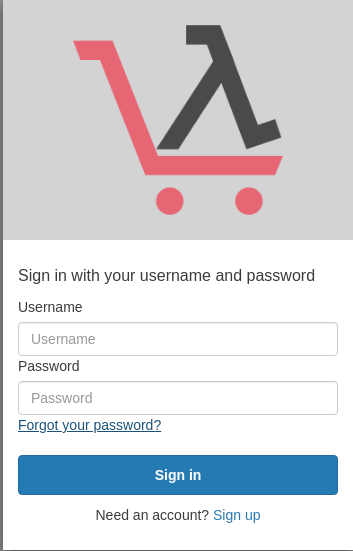
\includegraphics[scale=0.3]{../../../../Images/userManual/singIN.png}
    \centering
\end{figure}
User is redirected to the sign-up page. Here the user has to insert all his information in the form, all data is mandatory, and the sistem doesn't let the user continue unless he provides all information. \begin{figure}[!ht]
    \caption{Sign-in button}
    \vspace{10px}
    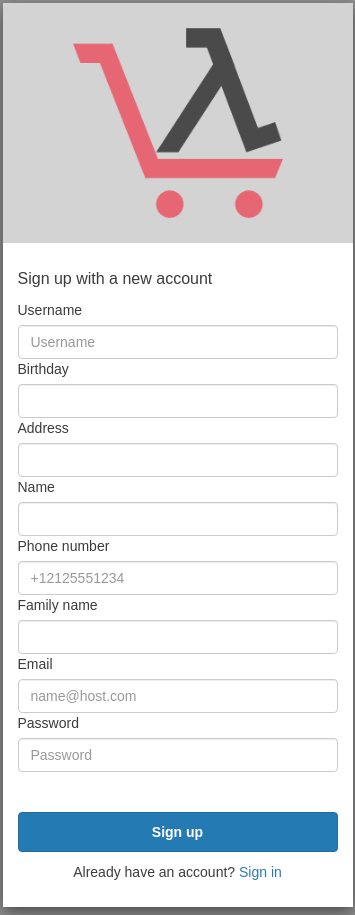
\includegraphics[scale=0.2]{../../../../Images/userManual/signUp.png}
    \centering
\end{figure}The password field must contain a lower case letter, an upper case letter, a special character, a number and has to be at least 8 characters long.
\begin{figure}[!ht]
    \caption{Sign-in button}
    \vspace{10px}
    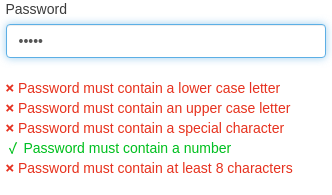
\includegraphics[scale=0.5]{../../../../Images/userManual/insertPWD.png}
    \centering
\end{figure}When the user fills in all the forms correctly he can press the \textit{sign-up} button, and he is redirected to the confermation page that asks a code.
\begin{figure}[!ht]
    \caption{Sign-in button}
    \vspace{10px}
    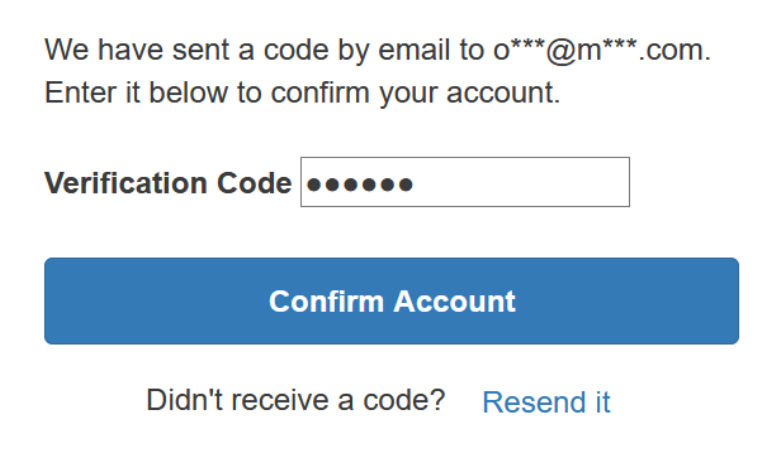
\includegraphics[scale=0.3]{../../../../Images/userManual/confermationCode.png}
    \centering
\end{figure}
The code is sent to the e-mail that the user provided in the previous step. When he recive the e-mail he can insert the code, and he can porced with the registration pressing the \textit{Confirm account} button. Afetr this the user has been successfully registered, and he is redirected to the home page.

\subsubsection{Sign-up error}
If any error happens during the registration procedure such as entering wrong data, you will be redirected to the previous section with an error message describing what the problem is.
\begin{figure}[!ht]
    \caption{Sign-in button}
    \vspace{10px}
    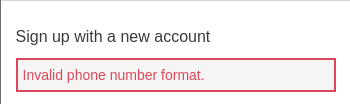
\includegraphics[scale=0.5]{../../../../Images/userManual/wrongData.png}
    \centering
\end{figure}
\subsection{Sign-in}
A user that has previously logged in to the platform can sign-in with his account. To perform this action the user has to click the \textit{sign-in/up} button present in the header.
\begin{figure}[!ht]
    \caption{Sign-in button}
    \vspace{10px}
    
\includegraphics[scale=0.5]{../../../../Images/userManual/signInButton.png}
    \centering
\end{figure}
When the button is pressed the is redirected to sign-in page provided by \textit{Amazon Cognito}. Here he can inset his data:
\begin{itemize}
    \item username;
    \item password.
\end{itemize}
\begin{figure}[!ht]
    \caption{Sign-in form}
    \vspace{10px}
    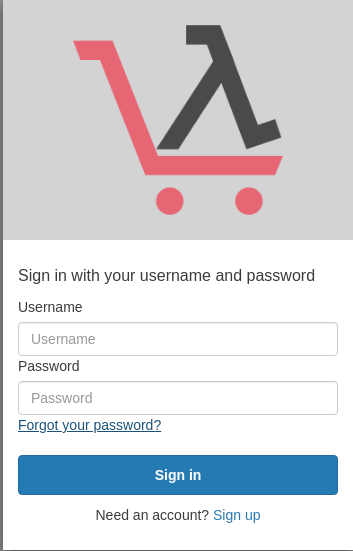
\includegraphics[scale=0.3]{../../../../Images/userManual/singIN.png}
    \centering
\end{figure}
\subsubsection{Login error}
If the user provides wrong credential a message error appeat to inform the user of the error.
\begin{figure}[!ht]
    \caption{Sign-in form}
    \vspace{10px}
    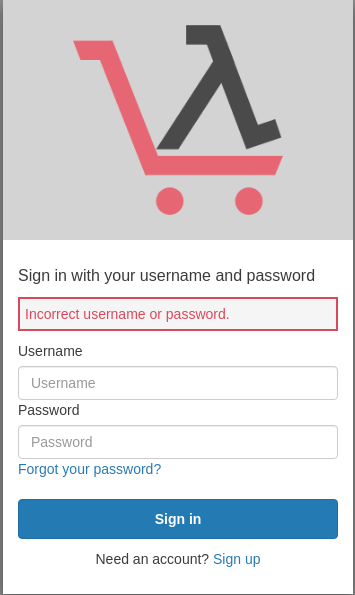
\includegraphics[scale=0.3]{../../../../Images/userManual/singInError.png}
    \centering
\end{figure}
\subsubsection{Forgetten password}
If a user forgot his password he can change it using the appropriate function. To achieve this the user has to open the \textit{forgot your password} link. After this he has to insert his username in the appropriate form.
\begin{figure}[!ht]
    \caption{Forgot password}
    \vspace{10px}
    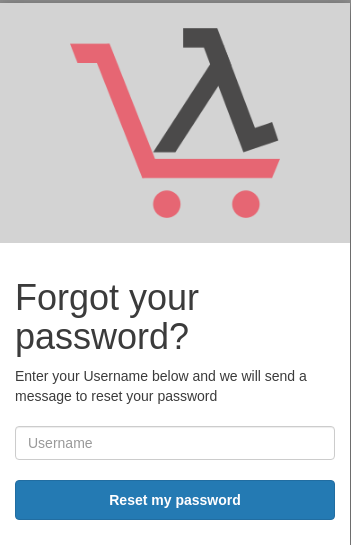
\includegraphics[scale=0.3]{../../../../Images/userManual/forgotPWD.png}
    \centering
\end{figure}
Whern this an e-mail with a verification code is sent to the e-mail used for the registration of the account. With this code the user can change his password using the provided form. When the user preses the confermation button the password is changed.
\begin{figure}[!ht]
    \caption{Change password form}
    \vspace{10px}
    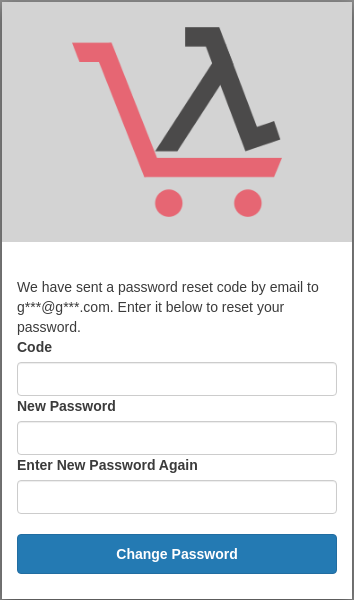
\includegraphics[scale=0.3]{../../../../Images/userManual/changingPWD.png}
    \centering
\end{figure}
\subsection{Browsing products}
A generic user can see the salable products. He can see these products in the Homepage sorted for products on sale and products in low quantity and in the product list page accessible from the \textit{products} button in the header, here the user can see all salable products.
\begin{figure}[!ht]
    \caption{Browsing products}
    \vspace{10px}
    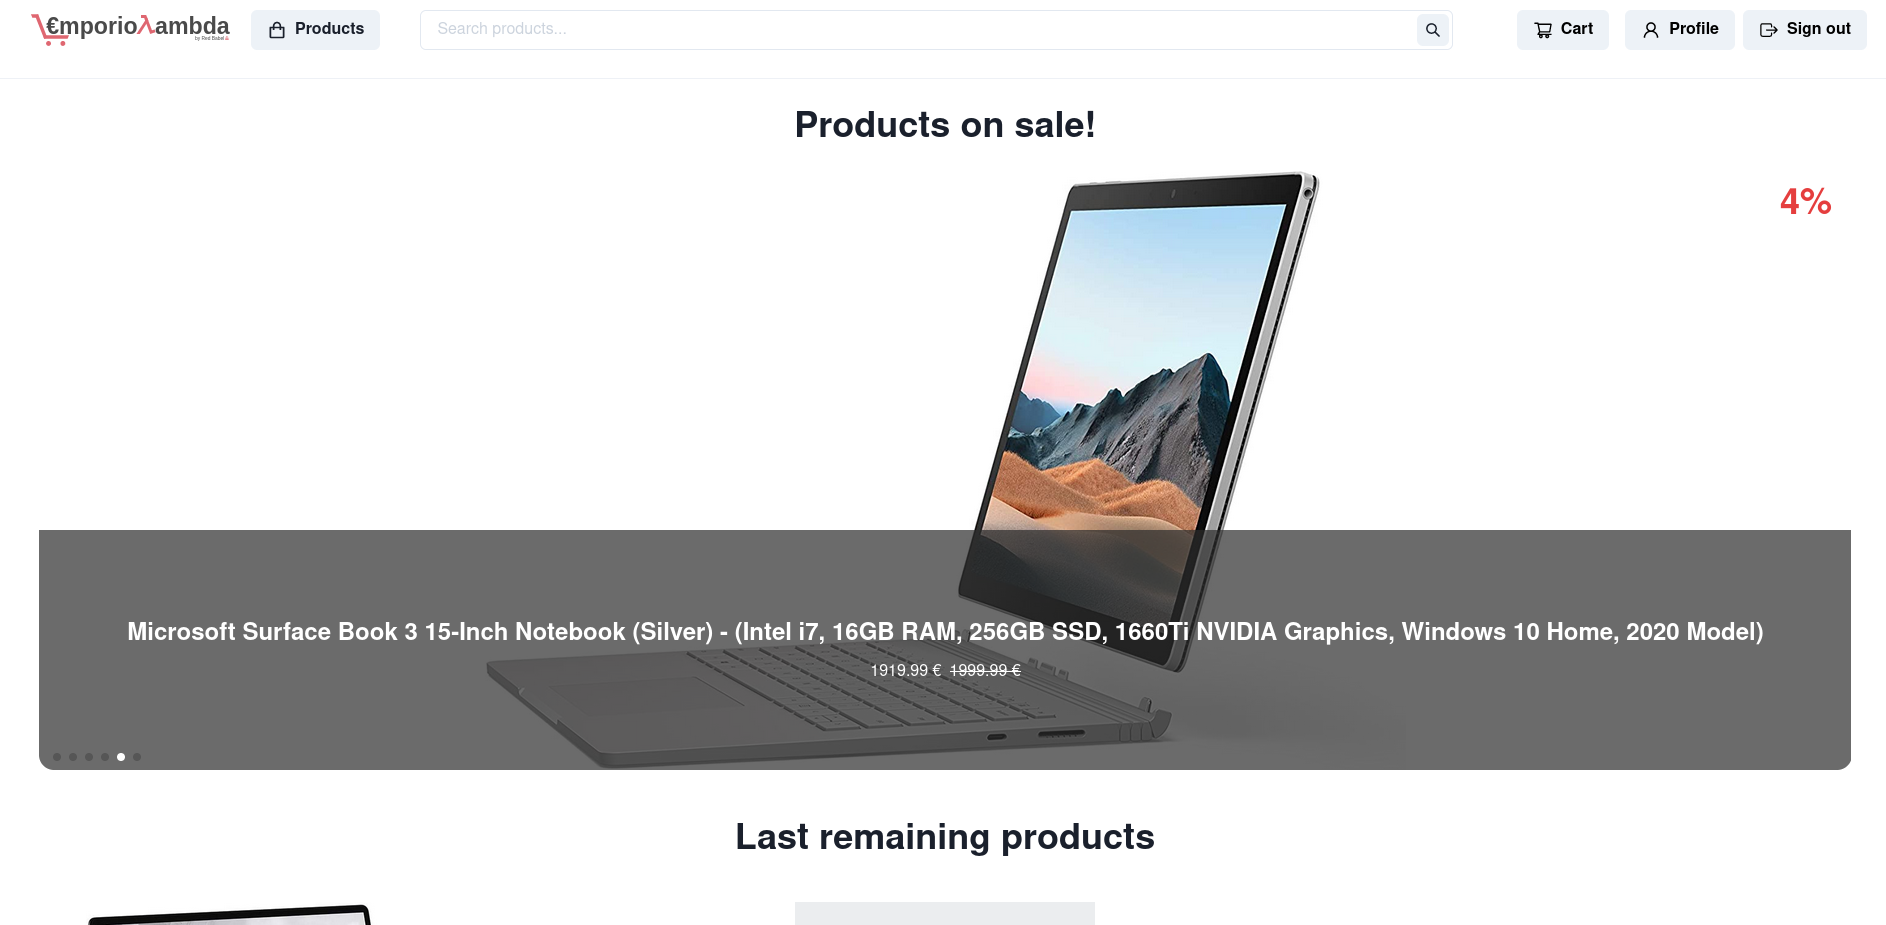
\includegraphics[scale=0.2]{../../../../Images/userManual/home.png}
    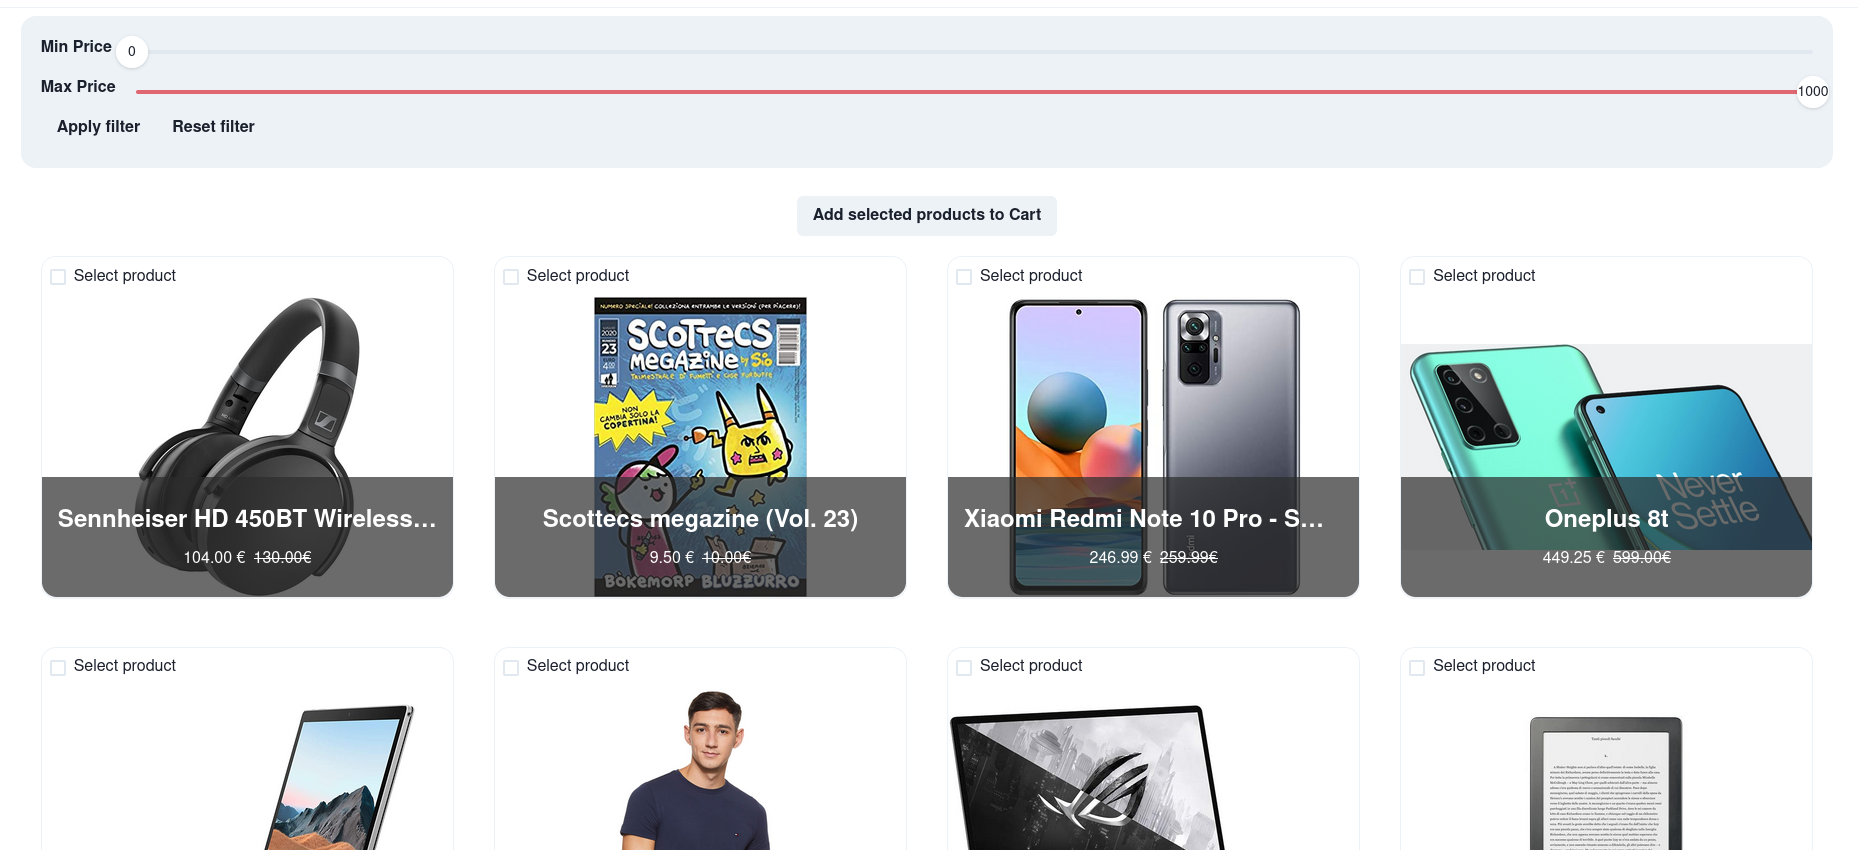
\includegraphics[scale=0.3]{../../../../Images/userManual/PLP.png}

    \centering
\end{figure}

\subsection{Searching and filtering products}
A generic user can search and filter products by price to achieve this he has to:
\begin{itemize}
    \item  \textit{Searching products}: the user can insert a keyword inside the searchbar in the header identifiable by the text \textit{Search products...} and press enter or clicking the search button identifiable by the search lens icon.
          \begin{figure}[!ht]
              \caption{Searching products}
              \vspace{10px}
              
\includegraphics[scale=0.2]{../../../../Images/userManual/searcbar.png}
              \centering
          \end{figure}
    \item \textit{Filtering by price}: the user inside the PLP using the slider on the top of the page can set the range of price with a minimun or maximum price or both, and after click \textit{Apply filter} button.
          \begin{figure}[!ht]
              \caption{Filter for products}
              \vspace{10px}
              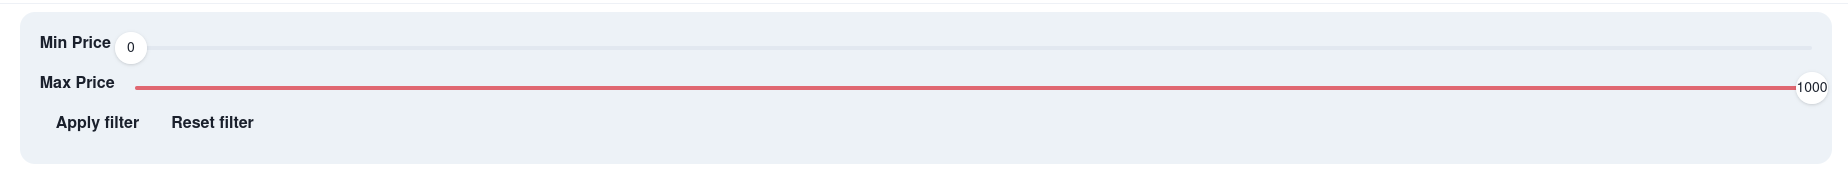
\includegraphics[scale=0.2]{../../../../Images/userManual/filter.png}
              \centering
          \end{figure}
\end{itemize}
\subsection{Viewing product detail}
To see the product detail a user has to press the product image, both in the home and in the PLP.
\begin{figure}[!ht]
    \caption{Product detail page}
    \vspace{10px}
    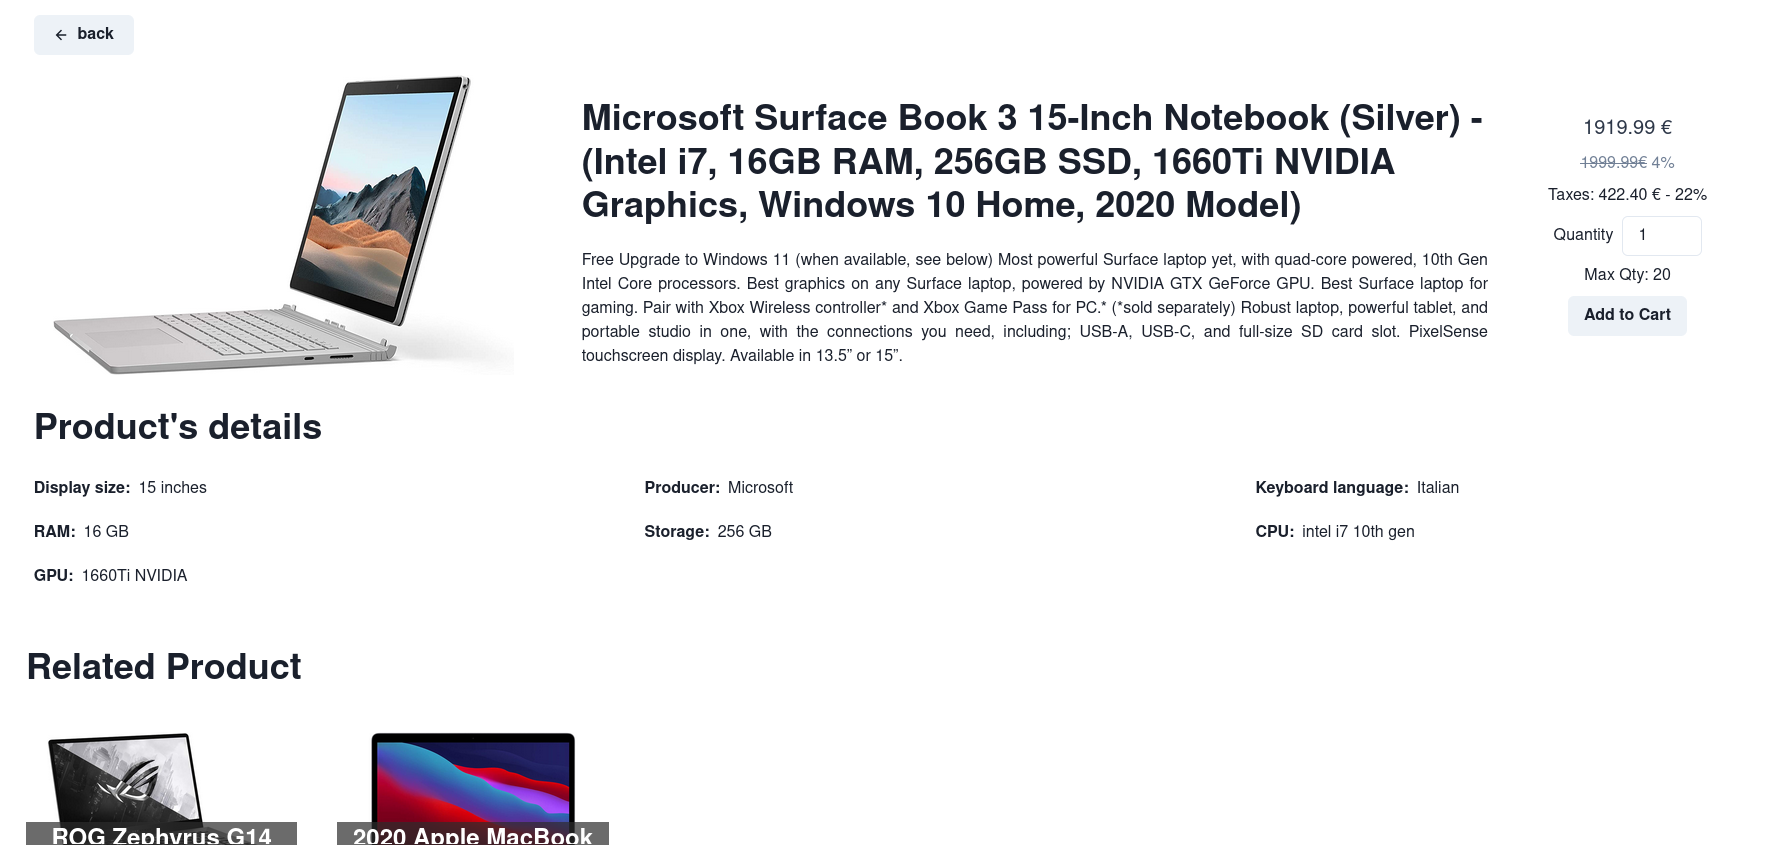
\includegraphics[scale=0.2]{../../../../Images/userManual/PDP.png}
    \centering
\end{figure}
He is redirected to the product detail page where he can see:
\begin{itemize}
    \item the product's title;
    \item the product's image;
    \item the product's description;
    \item the product's details;
    \item the product's price with the discounted price with the discount percentage if any ;
    \item the product's taxes;
    \item the product's availability;
    \item alternative produts.
\end{itemize}
\subsection{Adding products to the cart}
The user has two options to add products to the cart.
\begin{itemize}
    \item \textit{Directly from the product list page:} by seleting the products that he wants to add cart cheekcing the checkbox present in each of the product images, and clicking the \textit{add selected products to cart} button. In this way the user can add multiple porducts to the cart.
          \begin{figure}[!ht]
              \caption{Adding to cart multiple products}
              \vspace{10px}
              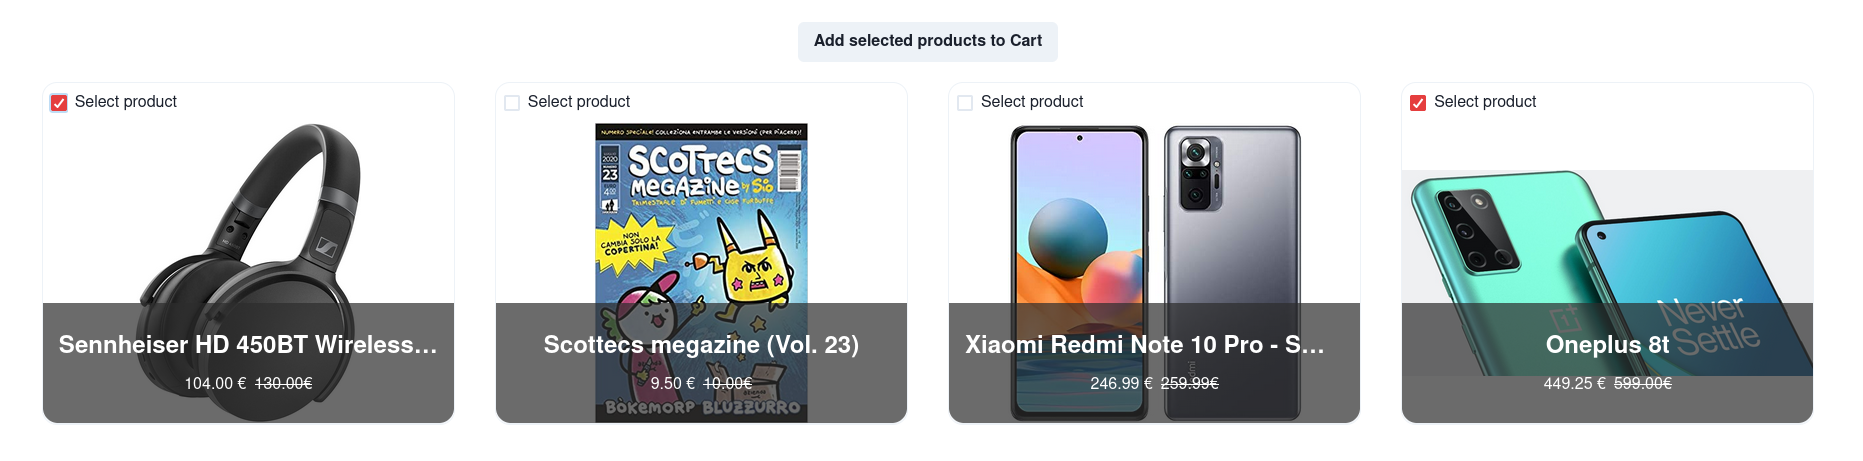
\includegraphics[scale=0.25]{../../../../Images/userManual/addtoCartPLP.png}
              \centering
          \end{figure}
    \item \textit{Form product's detail page:} When the user is in the detail page of a product he can add that product to the cart pressing the \textit{add to cart button} he can also set the quantity of products he wants to add to the cart.
          \begin{figure}[!ht]
              \caption{Adding to cart a product}
              \vspace{10px}
              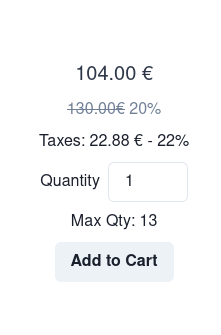
\includegraphics[scale=0.5]{../../../../Images/userManual/addToCartPDP.png}
              \centering
          \end{figure}
\end{itemize}
When the button is pressed a pop-up showing two buttons appears. One to continue to the cart and the other to return to the PLP page.
\begin{figure}[!ht]
    \caption{Add to cart result popup}
    \vspace{10px}
    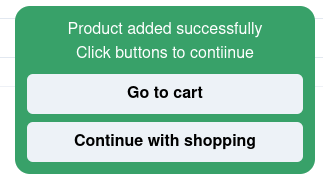
\includegraphics[scale=0.5]{../../../../Images/userManual/cartResult.png}
    \centering
\end{figure}
\subsection{Managing the cart}
A user can access the cart when he adds a product to the cart or by clicking the \textit{cart} button presnt in the header.
\begin{figure}[!ht]
    \caption{Cart page}
    \vspace{10px}
    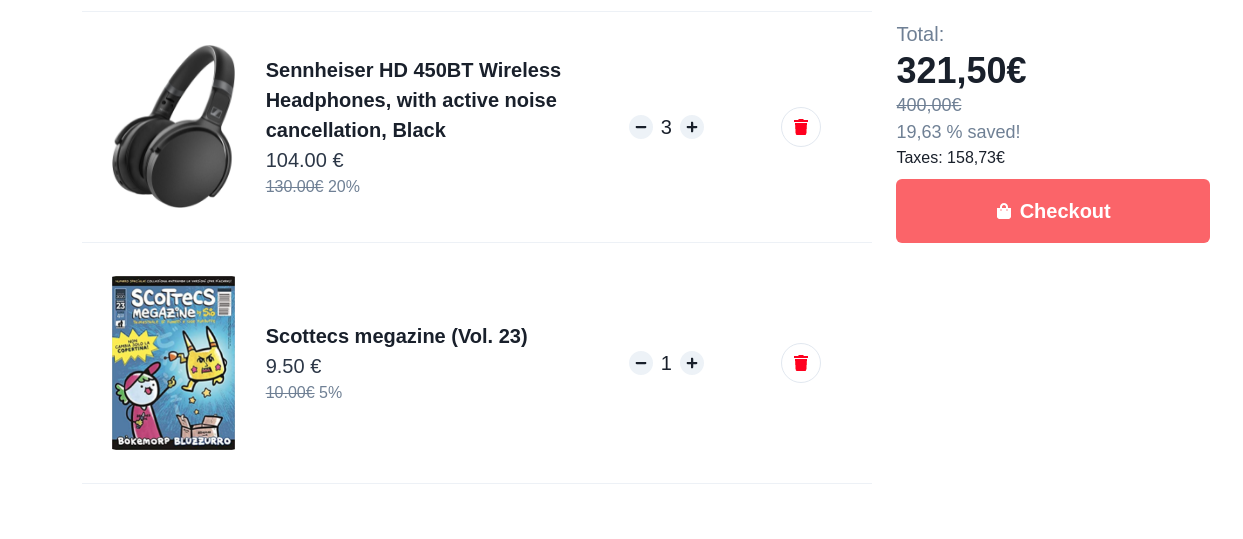
\includegraphics[scale=0.3]{../../../../Images/userManual/cart.png}
    \centering
\end{figure}
In the cart the user can see all the products that he previusly add to the cart. For each product he can see:
\begin{itemize}
    \item the product's title;
    \item the product's image;
    \item the product's description;
    \item the product's price and the discounted price with the discount percentage if any ;
    \item the product's quantity.
\end{itemize}
He can also manage the quantity by clicking the less or more buttons, to delete a product the user has to click the trash button. In the right part of the cart there is the cart summary where the user can see:
\begin{itemize}
    \item the cart's total price and the discounted price with the discount percentage if any ;
    \item the taxes of the entire cart.
\end{itemize}

